
% v2-acmsmall-sample.tex, dated March 6 2012
% This is a sample file for ACM small trim journals
%
% Compilation using 'acmsmall.cls' - version 1.3 (March 2012), Aptara Inc.
% (c) 2010 Association for Computing Machinery (ACM)
%
% Questions/Suggestions/Feedback should be addressed to => "acmtexsupport@aptaracorp.com".
% Users can also go through the FAQs available on the journal's submission webpage.
%
% Steps to compile: latex, bibtex, latex latex
%
% For tracking purposes => this is v1.3 - March 2012
\documentclass[prodmode,acmtecs]{acmsmall} % Aptara syntax
\usepackage[spanish,polish]{babel}
\usepackage[T1]{fontenc}
\usepackage{fancyvrb}
\usepackage{graphicx,hyperref}
\newcommand\cutout[1]{}


\usepackage[table]{xcolor}
\usepackage[utf8]{inputenc}
\usepackage[parfill]{parskip}
\usepackage{tabulary}
\PassOptionsToPackage{hyphens}{url}
\usepackage{hyperref}    
\usepackage[capitalize]{cleveref}


% Metadata Information
% !!! TODO: SET THESE VALUES !!!
\acmVolume{0}
\acmNumber{0}
\acmArticle{CFP}
\acmYear{0}
\acmMonth{0}

\newcounter{colstart}
\setcounter{page}{4}

\RecustomVerbatimCommand{\VerbatimInput}{VerbatimInput}%
{
%fontsize=\footnotesize,
fontfamily=\rmdefault
}


\newcommand{\UnderscoreCommands}{%\do\verbatiminput%
\do\citeNP \do\citeA \do\citeANP \do\citeN \do\shortcite%
\do\shortciteNP \do\shortciteA \do\shortciteANP \do\shortciteN%
\do\citeyear \do\citeyearNP%
}

\usepackage[strings]{underscore}



% Document starts
\begin{document}


\setcounter{colstart}{\thepage}

\acmArticle{CFP}
\title{\huge\sc SIGLOG Monthly 226}
\author{DAVID PURSER\affil{University of Warsaw, Poland}
\vspace*{-2.6cm}\begin{flushright}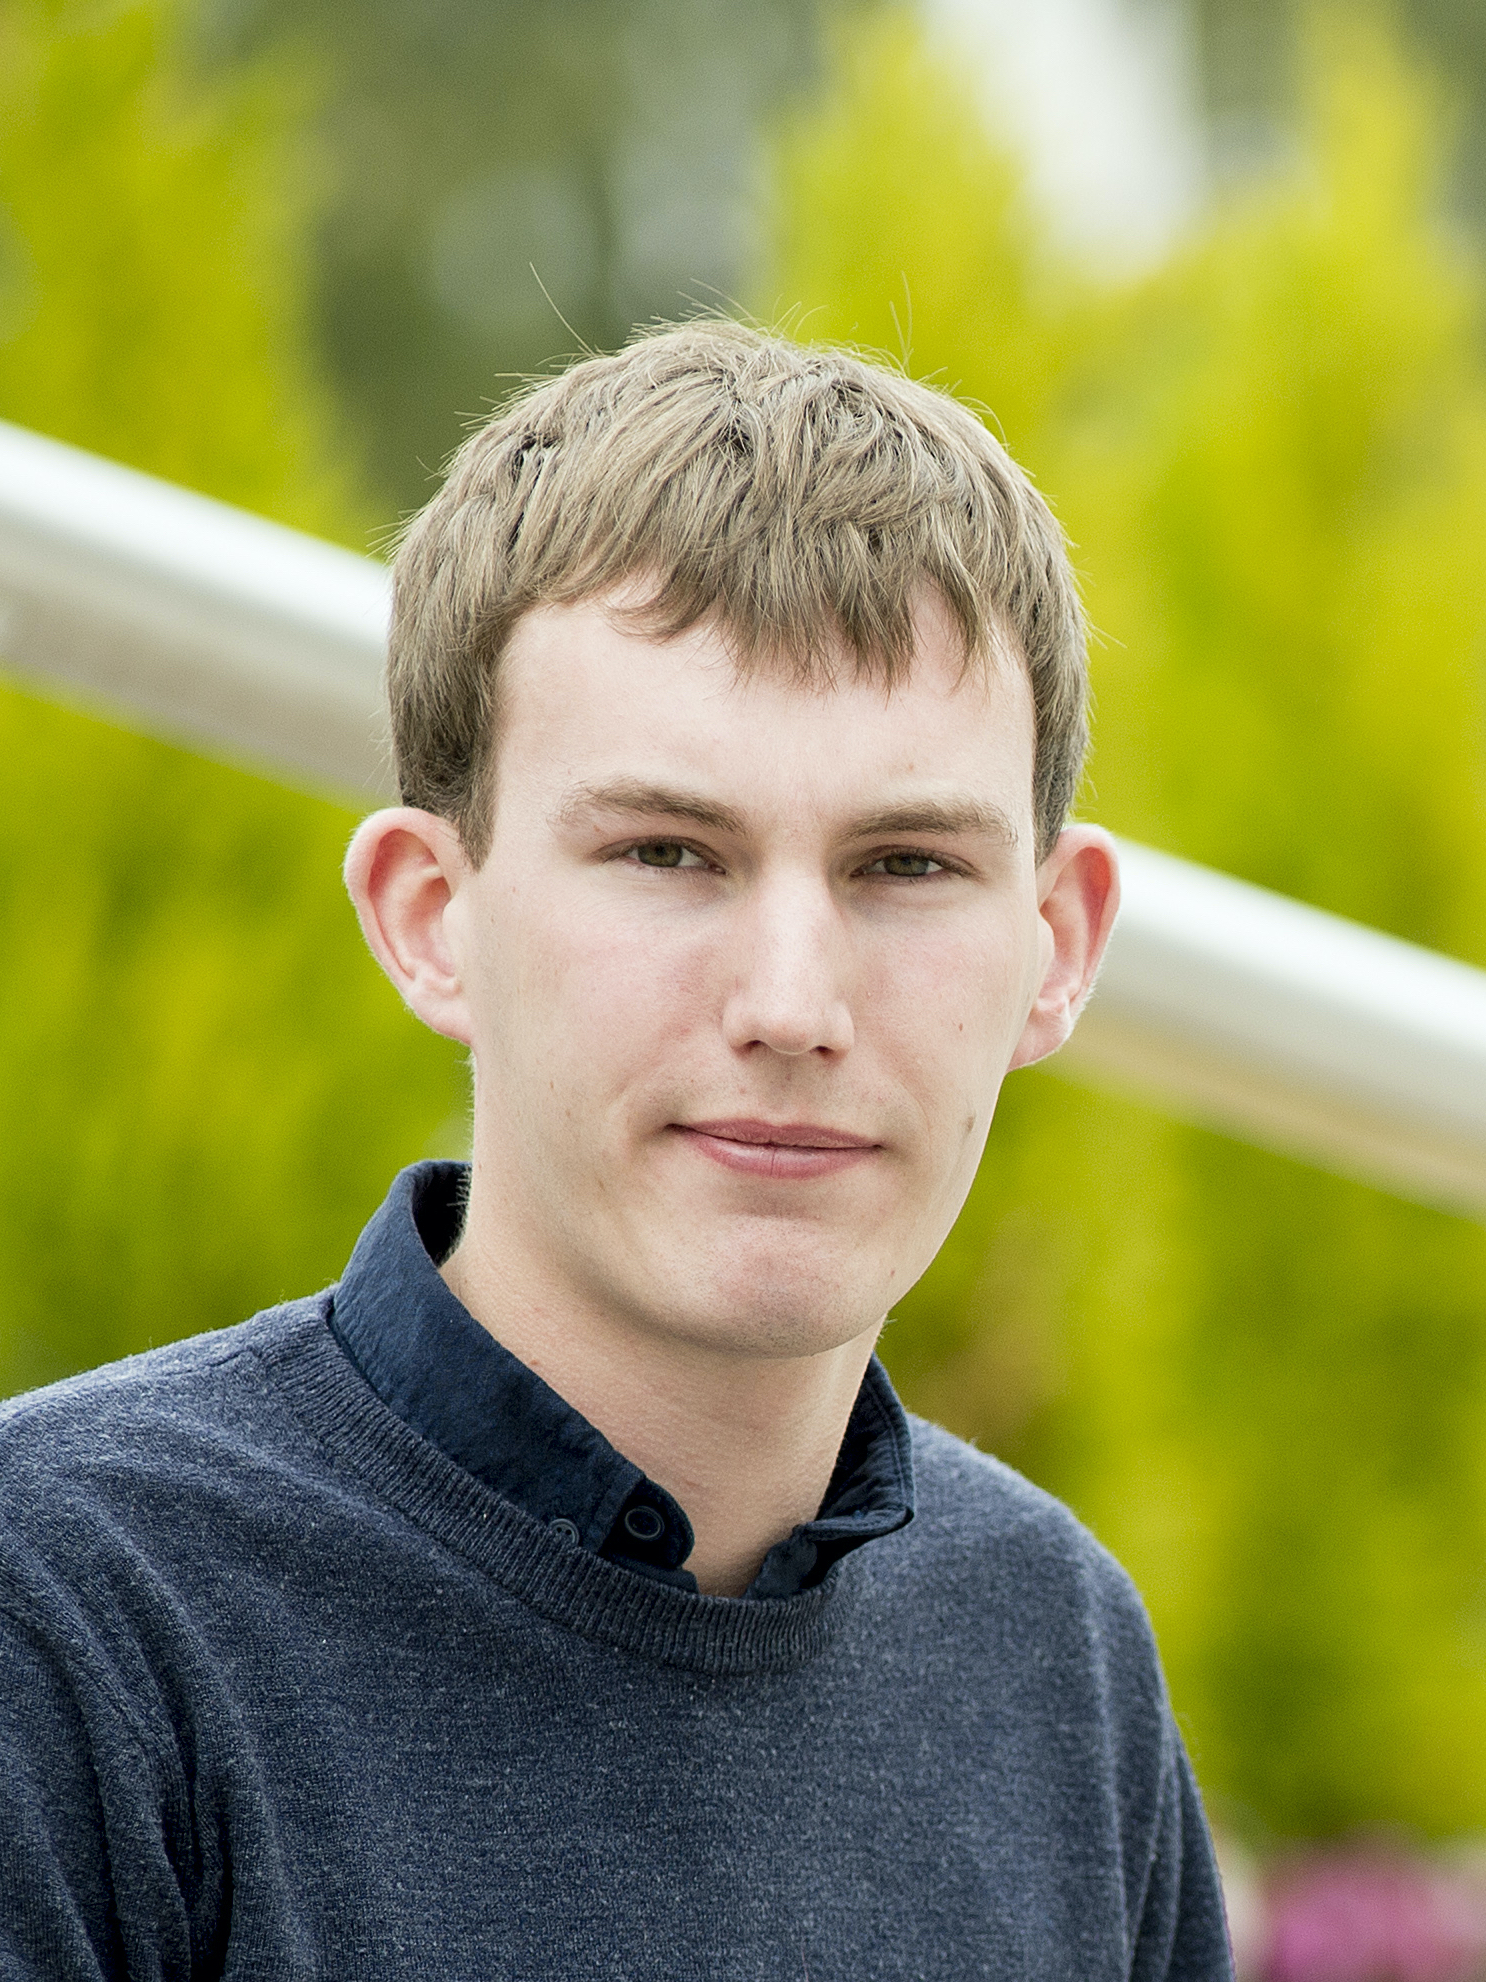
\includegraphics[width=30mm]{dp}\end{flushright}
}

\maketitlee

\href{https://lics.siglog.org/newsletters/}{Past Issues}
 - 
\href{https://lics.siglog.org/newsletters/inst.html}{How to submit an announcement}
\section{Table of Content}\begin{itemize}\item DEADLINES (\cref{deadlines}) 
 
\item SIGLOG MATTERS 
 
\begin{itemize}\item FLOC 2022 (\cref{FLOC2022})
\end{itemize} 
\item CALLS 
 
\begin{itemize}\item ACKERMANN AWARD 2022 (CALL FOR NOMINATIONS) (\cref{ACKERMANNAWARD2022})
\item TYPES 2022 and CA20111 (CALL FOR PARTICIPATION) (\cref{TYPES2022andCA20111})
\item Logic for the AI Spring Summer School (CALL FOR PARTICIPATION) (\cref{LogicfortheAISpringSummerSchool})
\item CiE 2022 (CALL FOR PARTICIPATION) (\cref{CiE2022})
\item ICALP 2022 (CALL FOR PARTICIPATION) (\cref{ICALP2022})
\item RCRA 2022 (CALL FOR PAPERS) (\cref{RCRA2022})
\item The ALP Alain Colmerauer Prolog Heritage Prize (CALL FOR NOMINATIONS) (\cref{TheALPAlainColmerauerPrologHeritagePrize})
\item AiML 2022 (CALL FOR PARTICIPATION) (\cref{AiML2022})
\end{itemize} 
\end{itemize}\section{Deadlines}\label{deadlines}\rowcolors{1}{white}{gray!25}\begin{tabulary}{\linewidth}{LL}TYPES 2022 and CA20111:  & Jun 01, 2022 (Early registration deadline) \\
GandALF 2022:  & Jun 03, 2022 (abstract, extended), Jun 10, 2022 (submission, extended) \\
PERR2022:  & Jun 04, 2022 (Submission, extended) \\
ESSLLI 2022:  & Jun 05, 2022 (Early bird registration, extended) \\
LAMAS\&SR 2022:  & Jun 06, 2022 (Paper, extended) \\
Logic for the AI Spring Summer School:  & Jun 15, 2022 (Student application) \\
FLOC 2022:  & Jun 20, 2022 (Early registration closed), Jul 20, 2022 (Regular registration closes) \\
FSCD 2024:  & Jun 27, 2022 (Deadline for proposals) \\
CiE 2022:  & Jun 30, 2022 (Regular registration) \\
Datalog 2.0 2022:  & Jul 01, 2022 (Paper registration), Jul 08, 2022 (Paper) \\
ACKERMANN AWARD 2022:  & Jul 01, 2022 (Deadline for nomination) \\
RCRA 2022:  & Jul 10, 2022 (Paper  deadline) \\
The ALP Alain Colmerauer Prolog Heritage Prize:  & Sep 02, 2022 (Deadline for nominations) \\
PODS 2023:  & Nov 28, 2022 (Second cycle abstract), Dec 05, 2022 (Full paper) \\
\end{tabulary}
\section{FLOC 2022: The Eighth Federated Logic Conference}\label{FLOC2022}  Jul 31-Aug 12, 2022, Haifa, Israel \\ 
  \href{https://www.floc2022.org/}{https://www.floc2022.org/}\\ 
CALL FOR PARTICIPATION 

\begin{itemize}\item  IMPORTANT INFORMATION 
 
\rowcolors{1}{white}{gray!25}\begin{tabulary}{\linewidth}{LL}Early registration closed:  & Jun 20, 2022 \\
Regular registration closes:  & Jul 20, 2022 \\
\end{tabulary}
 
  ON-SITE REGISTRATION will be possible during the conference. 
 
  The conference will take place IN PERSON, see \href{https://www.floc2022.org/covid-19}{https://www.floc2022.org/covid-19} for the latest COVID regulations. 
 
  It is imperative that you BOOK ACCOMMODATION ASAP to avoid disappointment. 
 
\begin{itemize}\item  Registration: \href{https://www.floc2022.org/registration}{https://www.floc2022.org/registration}
\item  Accommodation: \href{https://www.floc2022.org/accommodation}{https://www.floc2022.org/accommodation}
\end{itemize} 
  Registration for the main conference block gives you access to any other conference in the same period. Conference registration includes reception, lunches, and coffee breaks. A banquet ticket can be added to the conference registration. 
 
  Registration for a workshop day means you can attend any other workshop on the same day. Workshop registration includes lunches and coffee breaks. 
 
\item  ACCOMMODATION 
 
  \href{https://www.floc2022.org/accommodation}{https://www.floc2022.org/accommodation} 
 
  We have made block bookings at several locations in Haifa until mid-May and any unsold rooms are now being released. It is imperative that you book NOW to avoid disappointment, as July/August is a busy period in Haifa! 
 
\item  ABOUT FLOC 
 
  During the past forty years there has been extensive, continuous, and growing interaction between logic and computer science. In many respects, logic provides computer science with both a unifying foundational framework and a tool for modeling. In fact, logic has been called “the calculus of computer science”, playing a crucial role in diverse areas such as artificial intelligence, computational complexity, distributed computing, database systems, hardware design, programming languages, and software engineering. 
 
  The Federated Logic Conference brings together several international conferences related to mathematical logic and computer science and was first organized in 1996, as part of the DIMACS Special Year on Logic and Algorithms. Since then FLoC was held in Trento in 1999, Copenhagen in 2002, Seattle in 2006, Edinburgh in 2010, Vienna in 2014, and Oxford in 2018. 
 
  The eighth Federated Logic Conference (FLoC'22) will be held in Haifa, Israel, in July 2022. 
 
\item  CONFERNCES 
 
  FLoC 2022 brings together twelve major international conferences, 70+ workshops, and several special events. 
 
\begin{itemize}\item  CAV \href{http://i-cav.org/2022/}{http://i-cav.org/2022/}
\item  CP \href{https://cp2022.a4cp.org/}{https://cp2022.a4cp.org/}
\item  CSF \href{https://www.ieee-security.org/TC/CSF2022/}{https://www.ieee-security.org/TC/CSF2022/}
\item  DL \href{https://dai.fmph.uniba.sk/events/dl2022/}{https://dai.fmph.uniba.sk/events/dl2022/}
\item  FSCD \href{https://www.cs.tau.ac.il/~nachumd/FSCD/}{https://www.cs.tau.ac.il/~nachumd/FSCD/}
\item  ICLP \href{https://software.imdea.org/Conferences/ICLP2022/}{https://software.imdea.org/Conferences/ICLP2022/}
\item  IJCAR \href{https://easychair.org/cfp/IJCAR-2022}{https://easychair.org/cfp/IJCAR-2022}
\item  ITP \href{https://itpconference.github.io/ITP22/}{https://itpconference.github.io/ITP22/}
\item  KR \href{https://kr2022.cs.tu-dortmund.de/}{https://kr2022.cs.tu-dortmund.de/}
\item  NMR \href{https://sites.google.com/view/nmr2022/home-page}{https://sites.google.com/view/nmr2022/home-page}
\item  LICS \href{https://lics.siglog.org/lics22/}{https://lics.siglog.org/lics22/}
\item  SAT \href{http://satisfiability.org/SAT22/}{http://satisfiability.org/SAT22/}
\end{itemize} 
\item  KEYNOTES/PLENARY LECTURES 
 
\begin{itemize}\item  Catuscia Palamidessi, Director of Research at INRIA
\item  Don Knuth, CP invited speaker, The Art of Computer Programming at Stanford University
\item  Orna Kupferman, School of Computer Science and Engineering at The Hebrew University of Jerusalem
\item  Ziyad Hanna, Corporate Vice President at Cadence Design Systems
\item  Aarti Gupta, Department of Computer Science at Princeton University
\end{itemize} 
\item  CONFERENCE INVITED SPEAKERS 
 
\begin{itemize}\item  CAV: Arie Gurfinkel, Neha Rungta
\item  FSCD: Cynthia Kop, Alwen Tiu
\item  ICLP: Fabrizio Riguzzi, Theresa Swift
\item  LICS: Amal Ahmed, Mikolaj Bojanczyk
\item  KR: Yejin Choi, Tony Hunter, Leonid Libkin
\end{itemize} 
\item  SOCIAL EVENTS 
 
  There is one Reception and one Banquet during each FLoC block, and one Workshop Dinner during each of the workshop blocks. For details, see \href{https://www.floc2022.org/program}{https://www.floc2022.org/program}. Guests are welcome: you can reserve your place(s) via the registration system. 
 
\item  SPECIAL EVENTS 
 
  Two logic lounges are held - one on August 2nd and the other on August 7th. See \href{https://www.floc2022.org/logiclounge}{https://www.floc2022.org/logiclounge} for details. 
 
\item  MENTORING WORKSHOPS 
 
  Two mentoring workshops will be held, on August 1 and August 5. 
 
  See \href{https://www.floc2022.org/flocmentoringworkshop}{https://www.floc2022.org/flocmentoringworkshop} for more details. 
 
\item  SPONSORSHIP 
 
  We are indebted to our sponsors for making FLoC possible, see: \href{https://www.floc2022.org/sponsors}{https://www.floc2022.org/sponsors} 
 
\item  LOCAL INFORMATION 
 
  Our website includes details for travel (including accessibility), venues, and things to do in Haifa for our attendees and their families: see \href{https://www.floc2022.org/information}{https://www.floc2022.org/information} for more information. 
 
  FLoC 2022 promises to be an exciting meeting, and we hope to see you in Haifa! 
 
\item  CALL FOR VOLUNTEERS 
 
  FLoC 2022 invites students to apply to our volunteer program. Volunteers will receive a stipend (a variable amount towards registration and travel costs for students depending on the origin of travel) in exchange for volunteer work at the conference. FLoC’22 volunteers will be able to interact with speakers and participants, network with other researchers, and meet graduate students from all over the world. See \href{https://www.floc2022.org/volunteers}{https://www.floc2022.org/volunteers} for details. 
 
\item  ADDITIONAL INFORMATION 
 
  See \href{https://www.floc2022.org/about}{https://www.floc2022.org/about} 
 
\end{itemize}\section{ACKERMANN AWARD 2022: THE EACSL OUTSTANDING DISSERTATION AWARD FOR LOGIC IN COMPUTER SCIENCE}\label{ACKERMANNAWARD2022}CALL FOR NOMINATIONS 

\begin{itemize}\item  Nominations are now invited for the 2022 Ackermann Award. PhD dissertations in topics specified by the CSL and LICS conferences, which were formally accepted as PhD theses at a university or equivalent institution between 1 January 2020 and 31 December 2021 are eligible for nomination for the award. 
 
Deadline for nomination: Jul 01, 2022 
 
  Nominations can be submitted from 1 March 2022 and should be sent to the chair of the Jury, Thomas Schwentick, by e-mail: thomas.schwentick@tu-dortmund.de 
 
\item  THE AWARD  
 
  The 2022 Ackermann award will be presented to the recipient(s) at CSL 2023, the annual conference of the EACSL. 
 
  The award consists of 
 
\begin{itemize}\item  a certificate, 
\item  an invitation to present the thesis at the CSL conference, 
\item  the publication of the laudatio in the CSL proceedings, 
\item  an invitation to the winner to publish the thesis in the FoLLI subseries of Springer LNCS, and 
\item  financial support to attend the conference.
\end{itemize} 
  The jury is entitled to give the award to more (or less) than one dissertation in a year. 
 
\item  THE JURY 
 
  The jury consists of: 
 
\begin{itemize}\item  Christel Baier (TU Dresden); 
\item  Maribel Fernandez (King’s College London); 
\item  Jean Goubault-Larrecq (ENS Paris-Saclay); 
\item  Delia Kesner (IRIF, U Paris); 
\item  Slawomir Lasota (U Warsaw); 
\item  Prakash Panangaden (McGill University); 
\item  Simona Ronchi Della Rocca (University of Torino), the vice-president of EACSL; 
\item  Thomas Schwentick (TU Dortmund), the president of EACSL; 
\item  Alexandra Silva, (University College London), ACM SigLog representative; 
\item  James Worrell (U Oxford).
\end{itemize} 
\item  HOW TO SUBMIT  
 
  The candidate or his/her supervisor should submit 
 
\begin{itemize}\item  the thesis (ps or pdf file); 
\item  a detailed description (not longer than 10 pages) of the thesis in ENGLISH (ps or pdf file); it is recommended to not squeeze as much material as possible into these (at most) 10 pages, but rather to use them for a gentle introduction and overview, stressing the novel results obtained in the thesis and their impact; 
\item  a supporting letter by the PhD advisor and two supporting letters by other senior researchers (in English); supporting letters can also be sent directly to Thomas Schwentick (thomas.schwentick@tu-dortmund.de); 
\item  a short CV of the candidate; 5. a copy of the document asserting that the thesis was accepted as a PhD thesis at a recognized University (or equivalent institution) and that the candidate has received his/her PhD within the specified period.
\end{itemize} 
  The submission should be sent by e-mail as attachments to the chairman of the jury, Thomas Schwentick: thomas.schwentick@tu-dortmund.de 
 
  With the following subject line and text: 
 
\begin{itemize}\item  Subject: Ackermann Award 22 Submission 
\item  Text: Name of candidate, list of attachments
\end{itemize} 
  Submission can be sent via several e-mail messages. If this is the case, please indicate it in the text.  
 
\end{itemize}\section{TYPES 2022 and CA20111: 28th International Conference on Types for Proofs and Programs and EuroProofNet Cost Action meeting}\label{TYPES2022andCA20111}  Nantes, France, 20-25 June 2022 \\ 
  \href{https://types22.inria.fr}{https://types22.inria.fr}\\ 
  Early registration deadline: June, 1st 2022\\ 
  Registration: \href{https://types22.sciencesconf.org/registration/}{https://types22.sciencesconf.org/registration/}\\ 
CALL FOR PARTICIPATION 

\begin{itemize}\item  INVITED SPEAKERS 
 
\begin{itemize}\item  Youyou Cong: Composing Music from Types
\item  Ekaterina Komendantskaya: Refine and Synthesise: a type-theoretic view on neural network robustness.
\item  Sam Lindley: On the expressive power of types.
\item  Leonardo de Moura: The Lean 4 theorem prover and programming language
\end{itemize} 
\item  REGISTRATION FEES 
 
  To facilitate their attendance, TYPES'22 offers a reduced rate for students, available in the registration form. In addition, all registrations performed before June, 1st will be offered a discount. 
 
  It is possible to register for the satellite events only, which will take place on June 24th and 25th. Such a registration is free, but mandatory for catering purposes. Registering to TYPES'22 implicitly includes registration to satellite events. 
 
  See the registration page \href{https://types22.sciencesconf.org/registration/}{https://types22.sciencesconf.org/registration/} for details. 
 
\item  BACKGROUND 
 
  The TYPES meetings are a forum to present new and on-going work in all aspects of type theory and its applications, especially in formalised and computer assisted reasoning and computer programming. 
 
  The TYPES areas of interest include, but are not limited to: 
 
\begin{itemize}\item  foundations of type theory and constructive mathematics; 
\item  applications of type theory; 
\item  dependently typed programming; 
\item  industrial uses of type theory technology; 
\item  meta-theoretic studies of type systems; 
\item  proof assistants and proof technology; 
\item  automation in computer-assisted reasoning; 
\item  links between type theory and functional programming; 
\item  formalizing mathematics using type theory.
\end{itemize} 
  The EuroProofNet Cost Action CA20111 focuses on the same research topics as TYPES and partially sponsors the TYPES Conference.  
 
\end{itemize}\section{Logic for the AI Spring Summer School}\label{LogicfortheAISpringSummerSchool}  Lake Como School of Advanced Studies,\\ 
  September 12-16, 2022\\ 
  \href{https://lais.lakecomoschool.org/}{https://lais.lakecomoschool.org/}\\ 
CALL FOR PARTICIPATION 

\begin{itemize}\item  DESCRIPTION 
 
  Logic for the AI Spring aims at bringing together logicians and other scientists working around and within the currently blossoming new AI Spring. In addition to a glorious past which must not be forgotten, logic has a fundamental role to play, which is still largely in the making, in the future of AI research and applications. Researchers entering the field now have an opportunity to shape logic-based AI in the years to come. The School is designed to help them become culturally aware of the larger picture, which is made of urgent scientific and societal challenges, against which the unprecedented successes of the present AI Spring must be evaluated. 
 
\item  PROGRAMME \& TOPICS 
 
  The School will feature four 8-hour tutorials: 
 
\begin{itemize}\item  History and culture of AI (Stephanie Dick, Simon Fraser University)
\item  Combining Machine Learning and Theorem Proving (Josef Urban, Czech Institute of of Informatics, Robotics and Cybernetics)
\item  Multiagent Systems (Michel Wooldridge, Oxford University)
\item  Logic (Alessandra Palmigiano, VU Amsterdam)
\end{itemize} 
  A selection of participants will have an opportunity to present their own work in dedicated Work in Progress (WiP) sessions. The following is a (non exhaustive) list of topics in which we welcome WiP submissions: 
 
\begin{itemize}\item  Knowledge representation and reasoning in AI
\item  Logical methods in AI
\item  Uncertainty and decision-making in AI
\item  Computational social choice
\item  Explainable AI
\item  Human-compatible AI.
\end{itemize} 
\item  APPLICATION 
 
  Registration fees: 250 euro, VAT 22% included. The fee covers all lectures; course materials; lunches and coffee breaks; social dinner. 
 
\item  HOW TO APPLY 
 
  Details available at \href{https://lais.lakecomoschool.org/application/}{https://lais.lakecomoschool.org/application/} 
 
\item  DEADLINES: 
 
\rowcolors{1}{white}{gray!25}\begin{tabulary}{\linewidth}{LL}Student application:  & Jun 15, 2022 \\
Notification of acceptance:  & Jun 30, 2022 \\
Registration (only accepted students):  & Jul 10, 2022 \\
\end{tabulary}
 
\item  SUPPORT 
 
  Owing to generous funding from MOSAIC, HaPoC and Turing Center ETH we can offer limited financial support for particularly strong candidates who do not have access to funding. If you wish to apply for it, please send to hykel.hosni@unimi.it a letter stating your funding status. 
 
\item  PUBLICATION 
 
  The International Journal of Approximate Reasoning will publish a Special Issue to follow up on the themes covered in the School. Applicants are particularly encouraged to submit their original research to the SI (the usual refereeing procedure applies to guarantee the highest scientific standards). Deadlines to follow. 
 
\item  CO-LOCATED EVENT 
 
  On Saturday 17 September a one day workshop on “Bias, Risk and Opacity in AI” organised by members of the BRIO Research project (sites.unimi.it/brio) will take place at the Department of Philosophy, University of Milan. Participants to the Summer School are welcome to attend. A poster session for PhDs and Postdocs will be organised and School attendees are very welcome to present their current research (whether they have been selected or not for presentation at the Summer School). Please contact Giuseppe Primiero giuseppe.primiero@unimi.it for information. 
 
\item  CONTACTS 
 
  For enquiries about the venue of the school, travel, accommodation, and application procedure, please contact Alessandra Cazzaniga (alessandra.cazzaniga@fondazionealessandrovolta.it) at Fondazione Alessandro Volta, Como.  
 
\end{itemize}\section{CiE 2022: Computability in Europe 2022}\label{CiE2022}  Swansea, Wales, United Kingdom, CiE 2022 will be an on-site conference with some remote talks\\ 
  July 11-15, 2022\\ 
  \href{https://cs.swansea.ac.uk/cie2022/}{https://cs.swansea.ac.uk/cie2022/}\\ 
  Registration link: \href{https://easychair.org/register/register.cgi?a=28759463}{https://easychair.org/register/register.cgi?a=28759463}\\ 
CALL FOR PARTICIPATION 

\begin{itemize}\item  Computability in Europe 2022: Revolutions and revelations in computability 
 
\item  IMPORTANT DATES: 
 
Regular registration: Jun 30, 2022 
 
  Information about travel and accommodation is available at \href{https://cs.swansea.ac.uk/cie2022/travelandaccommodation}{https://cs.swansea.ac.uk/cie2022/travelandaccommodation} 
 
  CiE 2022 is the 18th conference organized by CiE (Computability in Europe), a European association of mathematicians, logicians, computer scientists, philosophers, physicists and others interested in new developments in computability and their underlying significance for the real world. 
 
\item  TUTORIAL SPEAKERS: 
 
\begin{itemize}\item  Dora Giammarresi (Università di Roma Tor Vergata)
\item  Noam Greenberg (Victoria University of Wellington)
\end{itemize} 
\item  INVITED SPEAKERS: 
 
\begin{itemize}\item  Erika Ábrahám (RWTH Aachen University)
\item  Thierry Coquand (University of Gothenburg)
\item  Liesbeth de Mol (Université de Lille)
\item  Damir Dzhafarov (University of Connecticut)
\item  Harvey Friedman (The Ohio State University)
\item  Svetlana Selivanova (Korea Advanced Institute of Science and Technology - KAIST)
\end{itemize} 
\item  SPECIAL SESSIONS: 
 
\begin{itemize}\item  At the intersection of computability and other areas of mathematics, organised by Denis Hirschfeldt (University of Chicago) and Karen Lange (Wellesley College)
\item  Computability theory of blockchain technology, organised by Arnold Beckmann (Swansea University) and Anton Setzer (Swansea University)
\item  Computing Language: Love Letters, Large Models and NLP, organised by Liesbeth de Mol (Université de Lille) and Giuseppe Primiero (University of Milan) for the Council of the HaPoC Commission
\item  Computing with bio-molecules, organised by Jérôme Durand-Lose (Université d'Orleans) and Claudio Zandron (University of Milan Bicocca)
\item  Constructive and reverse mathematics, organised by Samuele Maschio (Universita di Padova) and Takako Nemoto (Hiroshima Institute of Technology)
\item  Reachability problems, organised by Paul Bell (Liverpool John Moores University) and Igor Potapov (University of Liverpool)
\end{itemize} 
\item  See \href{https://cs.swansea.ac.uk/cie2022/}{https://cs.swansea.ac.uk/cie2022/} for further information 
 
\end{itemize}\section{ICALP 2022: The 49th International Colloquium on Automata, Languages, and Programming}\label{ICALP2022}  July 04-08  2022, in Paris, France, and online\\ 
CALL FOR PARTICIPATION 

\begin{itemize}\item  CONFERENCE 
 
  ICALP is the main conference and annual meeting of the European Association for Theoretical Computer Science (EATCS). As usual, ICALP will be preceded by a series of workshops, which will take place on July 4.  
 
  The 2022 edition has the following special features: 
 
\begin{itemize}\item  The conference is hybrid.
\item  This will be the 50th birthday of the conference and some special events are planned.
\item  The ICALP Extended Stay Support Scheme (IESSS) is here for helping the organisation of collaborations around the conference.
\end{itemize} 
  The 2022 edition will be also the occasion to celebrate the 50th anniversary of both EATCS and the first ICALP, which was first held in 1972 in Rocquencourt, in the Paris area. 
 
\item  IMPORTANT DATES AND INFORMATION  
 
  Website: \href{https://icalp2022.irif.fr/}{https://icalp2022.irif.fr/}  
 
\rowcolors{1}{white}{gray!25}\begin{tabulary}{\linewidth}{LL}Conference:  & July 04-08, 2022 \\
Workshops:  & Jul 04, 2022 \\
\end{tabulary}
 
  Early registration past, registration still possible 
 
\item  REGISTRATION  
 
  For registration, follow this link: \href{https://icalp2022.irif.fr/?page_id=50}{https://icalp2022.irif.fr/?page\_id=50} 
 
\item  EXTENDED STAY SUPPORT SCHEME (IESS)  
 
  For its 49th edition, the ICALP conference offers to its attendees an Extended Stay Support Scheme (IESSS) aiming at enhancing scientific collaborations and diminishing the carbon footprint of scientific research activities. ICALP 2022 attendees are encouraged to combine their visit to Paris with collaborations with local researchers. 
 
  This support scheme is primarily intended for participants travelling long distances and must be combined with an attendance to ICALP. Upon acceptation, research institutes involved in this mechanism will cover standard expenses (accommodation and traveling fees, plane excluded) and will provide material support for research activities. 
 
  See \href{https://icalp2022.irif.fr/?page_id=50}{https://icalp2022.irif.fr/?page\_id=50} for more information. 
 
\item  INVITED SPEAKERS  
 
\begin{itemize}\item  Albert Atserias, Universitat Politècnica de Catalunya 
\item  Constantinos Daskalakis, MIT 
\item  Leslie Ann Goldberg, Oxford University
\item  Madhu Sudan, Harvard 
\item  Stéphan Thomassé, ENS Lyon 
\item  Santosh Vempala, Georgia Tech
\end{itemize} 
\item  AWARDS  
 
   During the conference, the following awards will be given: 
 
\begin{itemize}\item  the EATCS award (\href{https://eatcs.org/index.php/eatcs-award}{https://eatcs.org/index.php/eatcs-award}),
\item  the Gödel prize (\href{https://eatcs.org/index.php/goedel-prize}{https://eatcs.org/index.php/goedel-prize}),
\item  the Presburger award (\href{https://eatcs.org/index.php/presburger}{https://eatcs.org/index.php/presburger}),
\item  the EATCS distinguished dissertation award (\href{https://eatcs.org/index.php/dissertation-award}{https://eatcs.org/index.php/dissertation-award}),
\item  the best papers for Track A and track B,
\item  the best student papers for Track A and track B.
\end{itemize} 
\item  ACCEPTED PAPERS  
 
  See \href{https://icalp2022.irif.fr/?page_id=85}{https://icalp2022.irif.fr/?page\_id=85}  
 
\item  WORKSHOPS  
 
  See \href{https://icalp2022.irif.fr/?page_id=46}{https://icalp2022.irif.fr/?page\_id=46} for more information. 
 
\begin{itemize}\item  Parameterized Approximation Algorithms Workshop 
\item  Combinatorial Reconfiguration 
\item  Recent Advances on Total Search Problems 
\item  Algorithmic Aspects of Temporal Graphs V 
\item  Trends in Arithmetic Theories 
\item  Structure Meets Power 2022 
\item  Straight-Line Programs, Word Equations and their Interplay 
\item  Graph Width Parameters: from Structure to Algorithms 
\end{itemize} 
\end{itemize}\section{RCRA 2022: 29th RCRA workshop on Experimental evaluation of algorithms for solving problems with combinatorial explosion }\label{RCRA2022}  affiliated to the 16th International Conference on Logic Programming and Non-monotonic Reasoning (LPNMR 2022) \href{https://sites.google.com/view/lpnmr2022}{https://sites.google.com/view/lpnmr2022} \\ 
  September, 5th, 2022; Genova, Italy \\ 
  RCRA group web site: \href{http://rcra.aixia.it/}{http://rcra.aixia.it/} Workshop web site: TBA e-mail: marco@dibris.unige.it, M.Vallati@hud.ac.uk\\ 
CALL FOR PAPERS 

\begin{itemize}\item   This event follows the series of the RCRA (Knowledge Representation and Automated Reasoning) annual meetings, held since 1994. The success of the previous events shows that RCRA is becoming a major forum for exchanging ideas and proposing experimentation methodologies for algorithms in Artificial Intelligence. 
 
\item  IMPORTANT DATES  
 
\rowcolors{1}{white}{gray!25}\begin{tabulary}{\linewidth}{LL}Paper submission deadline:  & Jul 10, 2022 \\
Notification of acceptance:  & Aug 01, 2022 \\
Final version of accepted original papers:  & Aug 22, 2022 \\
RCRA workshop:  & Sep 05, 2022 \\
\end{tabulary}
 
\item  AIMS AND SCOPE 
 
  Many problems in Artificial Intelligence show an exponential explosion of the search space. Although stemming from different research areas in AI, such problems are often addressed with algorithms that have a common goal: the effective exploration of huge state spaces. Many algorithms developed in one research area are applicable to other problems, or can be hybridized with techniques in other areas. Artificial Intelligence tools often exploit or hybridize techniques developed by other research communities, such as Operations Research. In recent years, research in Artificial Intelligence has more and more focused on experimental evaluation of algorithms, the development of suitable methodologies for experimentation and analysis, the study of languages and the implementation of systems for the definition and solution of problems. 
 
  Scope of the workshop is fostering the cross-fertilization of ideas stemming from different areas, proposing benchmarks for new challenging problems, comparing models and algorithms from an experimental viewpoint, and, in general, comparing different approaches with respect to efficiency, problem modeling, and ease of development. 
 
  Topics of interest include, but are not limited to: Experimental evaluation of algorithms for o knowledge representation o automated reasoning o planning o scheduling o machine learning o model checking o boolean satisfiability (SAT) o constraint programming o argumentation o temporal reasoning o combinatorial optimization o quantified boolean formulae and quantified constraints o modal logics o logic programming o answer set programming o ontological reasoning Definition and construction of benchmarks Experimentation methodologies Metaheuristics Algorithm hybridization Static analysis of combinatorial problems Languages and systems for definition and solution of problems Comparisons between systems and algorithms Application experiences (visualization, graphics, security, transports,...)  
 
\item  SUBMISSIONS 
 
  Authors are invited to submit either original and non-original papers. Publications showing negative results are welcome, provided that the approach was original and very promising in principle, the experimentation was well-conducted, the results obtained were unforeseeable and gave important hints in the comprehension of the target problem, helping other researchers to avoid unsuccessful paths. 
 
  Workshop submissions must be in PDF format, do not exceed 15 (for full papers) or 8 (for short papers) pages, and should be written in LaTeX, using the LNCS style.  
 
  \href{https://easychair.org/conferences/?conf=rcra2022}{https://easychair.org/conferences/?conf=rcra2022} 
 
  All submissions will be reviewed by at least three members of the program committee (TBD).  
 
\item  CONTACT  
 
  In case of need, the workshop co-chairs can be contacted by sending an email to: marco@dibris.unige.it, M.Vallati@hud.ac.uk  
 
\item  PROCEEDINGS 
 
  CEUR-WS Proceedings: Accepted original papers will be published in the AIxIA series of CEUR-WS AIIA Series on CEUR-WS.org (upon authors confirmation)  
 
  Moreover, as in some previous editions (\href{http://rcra.aixia.it/publications}{http://rcra.aixia.it/publications}), we are considering the possibility of having a special issue of an international journal, provided that a sufficient amount of high quality papers is collected. All technical papers, original and non-original, will be eligible. 
 
\end{itemize}\section{The ALP Alain Colmerauer Prolog Heritage Prize:}\label{TheALPAlainColmerauerPrologHeritagePrize}CALL FOR NOMINATIONS 

\begin{itemize}\item  The ALP Alain Colmerauer Prolog Heritage Prize is organized by The Association for Logic Programming (ALP) and The Prolog Heritage Association. 
 
\item  INTRODUCTION  
 
  In the summer of 1972, Alain Colmerauer and his team in Marseille developed and implemented the first version of the logic programming language Prolog. Together with both earlier and later collaborations with Robert Kowalski and his colleagues in Edinburgh, this work laid the practical and theoretical foundations for the Prolog and logic programming of today. Prolog and its related technologies soon became key tools of symbolic programming and Artificial Intelligence. 
 
  The Year of Prolog celebrates the 50th anniversary of these events and highlights the continuing significance of Prolog and Logic Programming both for symbolic, explainable AI, and for computing more generally. 
 
  This celebration will culminate with the award of the inaugural edition of the ALP Alain Colmerauer Prolog Heritage Prize for recent practical accomplishments that highlight the benefits of Prolog-inspired computing for the future.  
 
\item  ELIGIBILITY AND NOMINATIONS 
 
  Any individual or group of individuals can nominate themselves or their institution(s)/organization(s) for the Prize. The Prize will be given for depth, novelty, and proven or potential impact. A shortlist of up to five nominations will also be selected in the process. 
 
\rowcolors{1}{white}{gray!25}\begin{tabulary}{\linewidth}{LL}Deadline for nominations:  & Sep 02, 2022 \\
Notification of the shortlisted candidates:  & Sep 30, 2022 \\
\end{tabulary}
 
  For more information and details, see: \href{https://prologyear.logicprogramming.org/ColmerauerPrize.html}{https://prologyear.logicprogramming.org/ColmerauerPrize.html} 
 
\item  PRESENTATION OF THE AWARD 
 
  The Prize will be presented at the Prolog Day Symposium on November 10, 2022, in Paris, France. The winner(s) will receive a certificate and a cash Prize of 2,000 Euros. The expenses of the shortlisted nominees will be covered up to 1,000 Euros, supported by the Artificial Intelligence Journal. 
 
  The Year of Prolog and its activities, including the Alain Colmerauer Prize, are sponsored by the Association for Logic Programming, the Prolog Heritage Association, the AI Journal, Institut Carnot Cognition, and Institut Fredrik Bull, among others. 
 
\end{itemize}\section{AiML 2022: 14TH INTERNATIONAL CONFERENCE ON ADVANCES IN MODAL LOGIC}\label{AiML2022}  RENNES, Aug 22-25, 2022\\ 
  Registration now open\\ 
CALL FOR PARTICIPATION 

\begin{itemize}\item  Advances in Modal Logic is an initiative aimed at presenting the state of the art in modal logic and its various applications. The initiative consists of a conference series together with volumes based on the conferences. 
 
  AiML 2022 will be co-located with the Workshop on Logical Aspects of Multi-Agent Systems and Strategic Reasoning (LAMAS\&SR 2022).  
 
\item  REGISTRATION LINK 
 
  \href{https://aimllamassr2022.sciencesconf.org/}{https://aimllamassr2022.sciencesconf.org/} 
 
\item  WEBPAGES   
 
\begin{itemize}\item  AiML 2022: \href{https://aiml2022.irisa.fr/}{https://aiml2022.irisa.fr/}
\item  AiML Series: \href{http://www.aiml.net}{http://www.aiml.net}
\item  LAMAS\&SR: \href{https://lamassr.github.io/}{https://lamassr.github.io/}
\end{itemize} 
\item  TOPICS   
 
\begin{itemize}\item  history of modal logic
\item  philosophy of modal logic
\item  applications of modal logic
\item  computational aspects of modal logic
\item  theoretical aspects of modal logic
\item  specific instances and variations of modal logic
\end{itemize} 
\item  INVITED SPEAKERS 
 
\begin{itemize}\item  Willem Conradie, University of the Witwatersrand 
\item  Wesley Holliday, University of Berkeley 
\item  Francesca Poggiolesi, Sorbonne and CNRS 
\item  Rineke Verbrugge, University of Groningen (joint LAMAS\&SR speaker)
\end{itemize} 
\end{itemize}


To the \href{http://siglog.org/}{SIGLOG} or \href{https://lics.siglog.org}{LICS} website\end{document}